% This file was created with tikzplotlib v0.10.1.
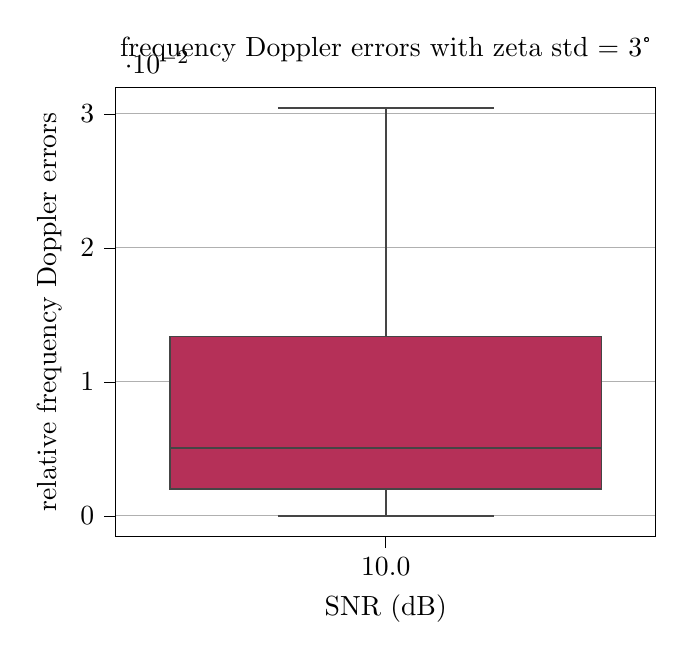
\begin{tikzpicture}

\definecolor{brown1814888}{RGB}{181,48,88}
\definecolor{darkgray176}{RGB}{176,176,176}
\definecolor{darkslategray69}{RGB}{69,69,69}

\begin{axis}[
tick align=outside,
tick pos=left,
title={frequency Doppler errors with zeta std = 3°},
x grid style={darkgray176},
xlabel={SNR (dB)},
xmin=-0.5, xmax=0.5,
xtick style={color=black},
xtick={0},
xticklabels={10.0},
y grid style={darkgray176},
ylabel={relative frequency Doppler errors},
ymajorgrids,
ymin=-0.00152059279460039, ymax=0.031941466853049,
ytick style={color=black}
]
\path [draw=darkslategray69, fill=brown1814888, semithick]
(axis cs:-0.4,0.00199899817573152)
--(axis cs:0.4,0.00199899817573152)
--(axis cs:0.4,0.0133725988409248)
--(axis cs:-0.4,0.0133725988409248)
--(axis cs:-0.4,0.00199899817573152)
--cycle;
\addplot [semithick, darkslategray69]
table {%
0 0.00199899817573152
0 4.09916656396567e-07
};
\addplot [semithick, darkslategray69]
table {%
0 0.0133725988409248
0 0.0304204641417922
};
\addplot [semithick, darkslategray69]
table {%
-0.2 4.09916656396567e-07
0.2 4.09916656396567e-07
};
\addplot [semithick, darkslategray69]
table {%
-0.2 0.0304204641417922
0.2 0.0304204641417922
};
\addplot [semithick, darkslategray69]
table {%
-0.4 0.00503832710257543
0.4 0.00503832710257543
};
\end{axis}

\end{tikzpicture}
